% Loki docker plugin causes all the containers to be unable to restart or kill. The alternative is to use the
% json-file driver with custom options. The json-file driver is the default driver for Docker.
% https://stackoverflow.com/questions/38567355/docker-compose-global-level-logging
% https://howchoo.com/devops/how-to-add-a-health-check-to-your-docker-container

\sect{Docker}{docker}
Docker es una plataforma software que permite el desarrollo, prueba y ejecución de aplicaciones de forma rápida y
cómoda, separando la aplicación de la infraestructura permitiendo ejecutar múltiples aplicaciones en un mismo servidor
(ver imagen~\ref{fig:docker-container-infrastructure}).\ Esto se realiza empaquetando la
aplicación, sus dependencias y otras herramientas necesarias para su ejecución en lo que se denominan
\boldFont{contenedores}, que son instancias ejecutables de una imagen de Docker.\ Las imágenes son ficheros de solo
lectura que contienen las instrucciones necesarias para crear un contenedor y normalmente se basan en otras imágenes
añadiendo o modificando configuraciones~\cite{docker-docs}.

\begin{figure}[ht]
	\centering
	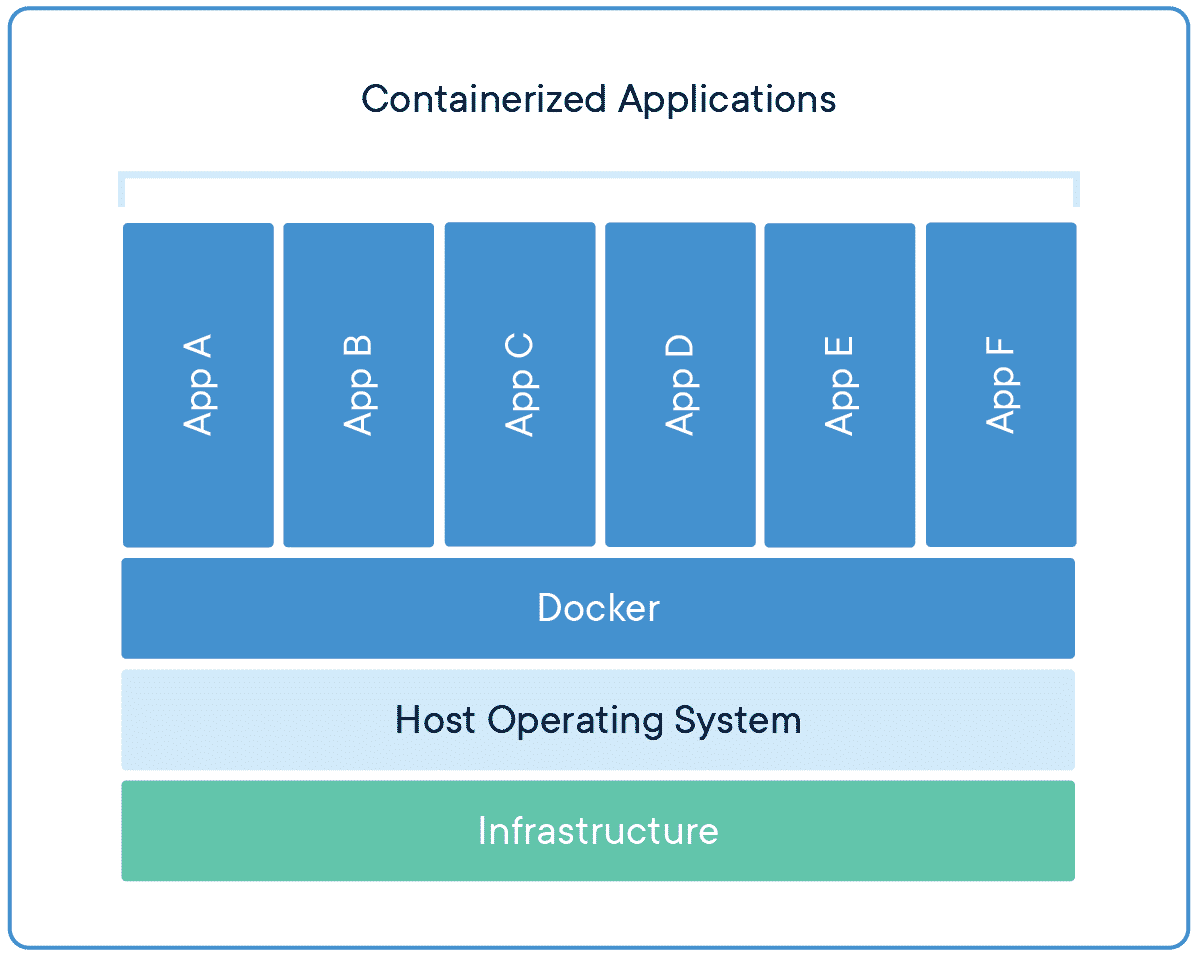
\includegraphics[width=0.8\textwidth]{res/images/container-what-is-container}
	\caption{Infrastructura docker. Fuente: \url{https://www.docker.com/resources/what-container}}
	\label{fig:docker-container-infrastructure}
\end{figure}

En el desarrollo de la aplicación se ha utilizado Docker para la creación de una imagen que contenga todo el código de
la aplicación así como las variables de entorno necesarias para su correcto funcionamiento.\ Se ha
utilizado la herramienta \monoFont{docker-compose}, que permite definir y ejecutar contenedores Docker de manera
sencilla.\ Para la configuración de los contenedores, se dispone del fichero \monoFont{docker-compose.yml} que se
encuentra en la raíz del proyecto y define los servicios que se ejecutarán en los contenedores, así como
las dependencias entre ellos.

Debido a que cada vez que se elimina un contenedor (al reiniciar el sistema o al generar de nuevo la imagen de la
aplicación para incluir cambios del código) se pierden los datos, la persistencia de los mismos y de sus
configuraciones es necesaria.\ Para lograr esto, se usan \boldFont{volúmenes}, que son directorios creados y
gestionados por Docker que se almacenan en el sistema de archivos del host, y que se montan en los contenedores cuando
se inicializan~\cite{docker-volumes}.\ De esta forma, los datos no se pierden al eliminar el contenedor.\ Los
volúmenes se definen en el mismo fichero \monoFont{docker-compose.yml} mediante la opción \monoFont{volumes} y son
los siguientes:

\begin{itemize}
	\item \monoFont{rschat-db}: contiene los datos y script inicial de la base de datos.
	\item \monoFont{rschat-logs}: contiene los ficheros de registro de la aplicación.
	\item \monoFont{grafana-storage}: contiene la configuración de Grafana.
\end{itemize}

A continuación, se mencionan todos los contenedores utilizados para la aplicación junto con una breve descripción de
cada uno de ellos:

	{\scriptsize Nota: los marcados con el símbolo \textsuperscript{\textasteriskcentered} se describirán en detalle
más adelante.}

\begin{itemize}
	\item \monoFont{rschat}: Contenedor que ejecuta el backend de la aplicación.
	\item \monoFont{rschat-db}: Contenedor que ejecuta la base de datos MySQL\@.
	\item \monoFont{prometheus\textsuperscript{\textasteriskcentered}}: Contenedor que ejecuta el servidor de métricas
	de Prometheus.
	\item \monoFont{grafana\textsuperscript{\textasteriskcentered}}: Contenedor que ejecuta el panel de observabilidad
	de Grafana.
	\item \monoFont{loki\textsuperscript{\textasteriskcentered}}: Contenedor que ejecuta el servidor de logs Loki.
	\item \monoFont{promtail\textsuperscript{\textasteriskcentered}}: Contenedor que ejecuta el agente de logs
	Promtail.
\end{itemize}
\label{itm:docker-compose-services}

\subsect{Prometheus (Métricas)}{prometheus}
Prometheus es un conjunto de herramientas de código abierto para la \boldFont{monitorización} de sistemas y
\boldFont{alertas} que recoge y
almacena las métricas con la marca de tiempo cuando se producen, incluyendo etiquetas (clave-valor) de manera
opcional~\cite{prometheus-overview}.
Estas métricas se utilizan para determinar el funcionamiento y estado de la aplicación en tiempo real, permitiendo
diagnosticar problemas de rendimiento o recursos de una manera rápida y sencilla.\ Para habilitar la exportación de
las métricas (de manera automática) por parte de la aplicación hay que realizar ciertas configuraciones,
que se detallan a continuación:

\begin{itemize}
	\item Añadir 2 librerías en el fichero \monoFont{pom.xml}~\cite{prometheus-metrics-pom}:
	\begin{itemize}
		\item spring-boot-starter-actuator
		\item micrometer-registry-prometheus
	\end{itemize}

	\item Para exponer el \quoted{endpoint} que permite ver las métricas, hay que añadir una propiedad en el fichero
	\monoFont{application.properties}:
	\begin{itemize}
		\item \monoFont{management.endpoints.web.exposure.include=prometheus}
	\end{itemize}

	\item Permitir las peticiones de tipo GET a \monoFont{/actuator/prometheus}: esto se configura
	de manera programática estableciendo la ruta como pública (permitiendo peticiones GET sin necesidad de estar
	autenticado).
\end{itemize}
\label{itm:metrics-export-config}

Las métricas que más se utilizarán son las relacionadas con el rendimiento de la aplicación y el uso de recursos del
sistema, aunque se han añadido algunas personalizadas para determinar el uso que se hace de determinadas partes de la
aplicación.\ La lista con las métricas más usadas es la siguiente:

\begin{itemize}
	\item jvm\_memory\_used\_bytes: bytes usados por la JVM\@.
	\item jvm\_memory\_committed\_bytes: bytes que se están guardando en el \quoted{heap} de la JVM\@.
	\item system\_cpu\_usage: uso de CPU del sistema.
	\item process\_cpu\_usage: uso de CPU por parte de la aplicación.
	\item system\_cpu\_count: número de procesadores físicos utilizados en todo el sistema.
	\item logback\_events\_total: número de eventos de log de un determinado nivel (info, debug, warn, error).
	\item http\_server\_requests\_seconds\_count: número de peticiones HTTP realizadas a la aplicación.
	\item jvm\_threads\_live\_threads: número de hilos en ejecución.
	\item jvm\_threads\_daemon\_threads: número de hilos en ejecución (en segundo plano).
	\item jvm\_threads\_peak\_threads: número máximo de hilos.
\end{itemize}
\label{itm:most-used-metrics}

\subsect{Grafana (Panel de observabilidad)}{grafana}
Grafana es una solución de código abierto para mostrar las analíticas que se recogen de las aplicaciones de una
manera amigable en paneles personalizables~\cite{what-is-grafana}.\ Permite estudiar, analizar y monitorizar
aplicaciones a lo largo del tiempo gracias a las marcas de tiempo proporcionadas junto con los datos que se
recolectan.\ Se puede conectar con muchas fuentes de datos, como Graphite, Prometheus, ElasticSearch, MySQL, etc.\
Una ventaja de Grafana es que ofrece una solución \quoted{on-premise}, que permite desplegar una instancia propia en
el mismo servidor donde se ejecuta la aplicación.\ De esta manera, se garantiza la seguridad y protección de los
datos, ya que no se exponen a Internet de manera directa.

Para la configuración de Grafana en el entorno de producción, se necesita un contenedor Docker que utilice la imagen
\monoFont{grafana/grafana-oss} y exponga un puerto para permitir conexiones desde hosts externos a la red interna.\ A
continuación, se presenta la configuración básica para ejecutar una instancia de Grafana:

\begin{codeBlock}
	\begin{minted}[
		baselinestretch=1.1,
		fontsize=\footnotesize,
		tabsize=2,
	]{yaml}
version: '3.7'
services:
  grafana:
    image: grafana/grafana-oss:9.3.1
    ports:
      - "4046:3000"
    expose: [ 4046 ]
    volumes:
      - grafana-storage:/var/lib/grafana
    env_file:
      - ./env/.env.grafana
    networks:
      - rschat-net
	\end{minted}
	\caption{Configuración mínima para ejecutar un contenedor con Grafana}
\end{codeBlock}

\subsect{Loki (Servidor de logs)}{loki}

\subsect{Promtail (Agente de logs)}{promtail}
